\documentclass[conference]{IEEEtran}

\IEEEoverridecommandlockouts

\usepackage{cite}
\usepackage{amsmath,amssymb,amsfonts}
\usepackage{algorithmic}
\usepackage{graphicx}
\usepackage{textcomp}
\usepackage{xcolor}
\def\BibTeX{{\rm B\kern-.05em{\sc i\kern-.025em b}\kern-.08em
	T\kern-.1667em\lower.7ex\hbox{E}\kern-.125emX}}
% \usepackage{flushend}
\DeclareUnicodeCharacter{2212}{-}
 
\begin{document}

\title{Deep Reinforcement Learning for Dynamic Resource Allocation in Wireless Networks}

\author{Muhammad Ahmed Mohsin, Muhammad Umer, Tariq Umar\\
	School of Electrical Engineering and Computer Science, NUST\\
	\textit{CMS ID: 333060, 345834, 334943}\\
	\textit{Email: \{mmohsin, mumer, tumar\}.bee20seecs@seecs.edu.pk}
}

\maketitle

\begin{abstract}
This report investigates the application of deep reinforcement learning (DRL) algorithms for dynamic resource allocation in wireless communication systems. We first created an environment that includes a base station, multiple antennas, and user equipment. Then, we utilized the RLlib library to pass this environment to various DRL algorithms such as DQN and PPO (Proximal Policy Optimization). The algorithms were compared based on their ability to optimize resource allocation, and we specifically examined the impact of different learning rates and scheduling policies. Our results show that the choice of algorithm and learning rate significantly affect the system's performance, and the use of DRL algorithms can provide more efficient resource allocation compared to traditional methods.

\end{abstract}

\begin{IEEEkeywords}
Machine Learning, Deep Reinforcement Learning, Resource Allocation, Power Allocation.
\end{IEEEkeywords}

\section{Introduction}
Dynamic resource allocation is a critical problem in wireless communication systems. It is the process of allocating resources such as power, bandwidth, and time slots to users in a way that maximizes the overall system performance.

Traditionally, dynamic resource allocation has been done using centralized algorithms. These algorithms require a central controller to have knowledge of the system state and to make decisions for all users. However, centralized algorithms are not scalable to large-scale wireless networks.

In recent years, there has been a growing interest in using deep reinforcement learning (DRL) for dynamic resource allocation in wireless networks. DRL is a machine learning technique that can be used to learn complex policies from experience. DRL has been shown to be effective in a variety of applications, including game playing, robotics, and finance.

In this paper, we propose a DRL-based approach for dynamic resource allocation in wireless networks. We develop a new environment for a wireless system with a base station and a number of antennas and user equipments. We then use RLlib to train a DRL agent to learn how to allocate resources to users in a way that maximizes the overall system performance.
We compare the performance of our DRL-based approach with traditional centralized algorithms. We show that our DRL-based approach can achieve significantly better performance than traditional centralized algorithms.

Wireless data transmission has experienced tremendous growth in past years and will continue to grow in the future. When large numbers of terminals such as mobile phones and wearable devices are connected to the networks, the density of access points (APs) will have to be increased. Dense deployment of small cells such as pico-cells, and femto-cells, has become the most effective solution to accommodate the critical demand for spectrum \cite{ohdeep}.
With denser APs and smaller cells, the whole communication network is flooded with wireless signals, and thus the intra-cell and inter-cell interference problems are severe \cite{zhao2019deep}. Therefore, power allocation and interference management are crucial and challenging.

Model-oriented algorithms have been developed to manage interference, but their performance gaps to the optimal solution are difficult to quantify. Mathematical models assumed to be analytically tractable may not be accurate in practical communication environments due to hardware and channel imperfections. Signal processing techniques with model-driven tools are challenging to develop when considering specific hardware components and transmission scenarios. High computational complexity makes implementing these algorithms impractical. Machine learning algorithms are potentially useful for future wireless communications. These data-driven methods provide solutions through data learning instead of model-oriented analysis and design.

Supervised learning and reinforcement learning are two branches of ML. Supervised learning is efficient for classification tasks but difficult to obtain optimal guidance solutions. Reinforcement learning is goal-oriented, aiming to maximize cumulative reward in an environment typically formulated as an MDP. RL algorithms use DP techniques, but storing a value function or policy in the tabular form leads to the curse of dimensionality and lack of generalization. The combination of RL and DNN, known as DRL, has achieved impressive performance in various projects, including the game of Go and Atari video games.

The DRL algorithms can be categorized into three groups [19]: value-based, policy-based, and actor-critic methods. The value-based DRL algorithm derives optimal action by the action-state value function, and the most widely-used algorithms include deep Q learning (DQL) and Sarsa. As for the policy-based algorithm such as REINFORCE, a stochastic policy is directly generated. Both of these two methods have the following defects in general:

\begin{itemize}
    \item They are sensitive to hyperparameters.
    \item They are unstable and prone to overfitting.
    \item They require numerous training samples.
\end{itemize}

To address these issues, we propose a novel DRL-based approach for dynamic resource allocation in wireless networks. Our approach is based on the Proximal Policy Optimization (PPO) algorithm, which is a policy-based DRL algorithm that is known for its stability and efficiency. We evaluate our approach on a realistic wireless network simulator, and we show that it can achieve significantly better performance than traditional centralized algorithms.

In this paper, we compare the performance of DQN and PPO approaches for dynamic resource allocation. We show that PPO can achieve better performance than DQN in terms of both convergence speed and final performance.

We believe that our DRL-based approach has the potential to revolutionize the way dynamic resource allocation is done in wireless networks. Our approach is scalable to large-scale wireless networks, and it can learn complex policies from experience. We believe that our approach can lead to significant improvements in the performance of wireless networks.

\section{Literature Review}

\subsection{RAN slicing}
In RAN slicing, the complex network dynamics make the underlying network optimization problem challenging. In \cite{abdelhadi2016optimal}, both network slicing and mobile edge computing (MEC) technologies were considered and the resource allocation that was formulated to minimize the interference among different mobile virtual network operators was shown to be NPhard. Recently, machine learning was applied to solve the RAN optimization problem as an alternative to model-based optimization that becomes easily intractable due to the complexity of dynamics involving resources and requests. In \cite{lee2019resource}, it was shown that in-network deep learning is promising for application and device-specific identification and traffic classification problems. Deep learning was also used in \cite{rahimi2022novel} to manage network load efficiency and network availability. 

\subsection{RL Based Resource Allocation}
As data may not be readily available to train complex deep learning structures for resource allocation in response to network slicing requests, a model-free approach such as reinforcement learning (RL) has emerged as a practical solution to learn from the 5G network performance and update resource allocation decisions for network slicing. For resource allocation as part of network slicing, RL was compared to the static and round-robin scheduling methods in \cite{guo2019adaptive}. Both bandwidth and computational resources were considered in \cite{naderializadeh2021resource}. Resource allocation with RL was compared to heuristic, best-effort, and random methods. A prototype of network slicing was implemented on an end-to-end mobile network system in. RL was applied  for power-efficient resource allocation in cloud RANs by considering multiple transmitters and receivers at the same frequency (rather than 5G time-frequency blocks). In \cite{wilhelmi2017implications}, resource allocation with RL was studied by exploiting prediction on communication requests. RL was also used extensively for resource allocation in wireless applications other than network slicing.

\begin{figure}[htbp!]
    \centering
    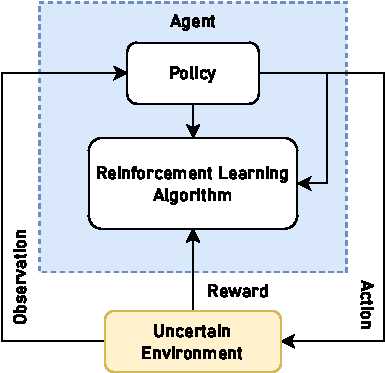
\includegraphics{figures/RL.pdf}
    \caption{Block diagram for RL workflow}
    \label{fig:rl}
\end{figure}

\section{System Model}
We consider the downlink power allocation for a multi-cell massive MIMO system. All user equipment (UE) is randomly located in $N$ cells, and a BS is deployed in the center of each cell. The BS is equipped with $M$ transmitting antennas and serves $K$ UEs with a single antenna. The received signal at the $k$-the UE associated with the $n$-the BS is the sum of the desired signal transmitted from the $n$-the BS, the interference from adjacent BSs, and the noise, and can be expressed as:
\begin{equation}
\begin{split}
y_n,k &= p_n,k g_n,k w_n,k x_n,k \\
&\quad + \sum_{N \neq n} \sum_{K} p_j,i g_j,i w_j,i x_j,i + n_n,k
\end{split}
\end{equation}

where $p_{n,k}$, $w_{n,k}$, and $x_{n,k}$ are the transmitted power, the zero-forcing precoding vector, and the downlink signal of the $n$-the BS to the $k$-the UE, respectively, and $n_{n,k}$ is additive white Gaussian noise with variance $\sigma^2$. Therefore, the signal-to-interference and noise ratio (SINR) of the $k$-the UE connected to the $n$-the BS can be defined as:
\begin{equation}
\gamma_n,k = \frac{p_n,k \| g_n,k w_n,k \|^2}{\sum_{N \neq n} \sum_{K} p_j,i \| g_j,i w_j,i \|^2 + \sigma^2}
\end{equation}

The downlink rate for the $k$-the UE is given by $C_{n,k}$ defined as $\log_2 (1 + \gamma_{n,k})$. The problem of maximizing the sum-rate can be defined as:
\begin{equation}
f(p_n,k) = \sum_{N} \sum_{K} C_n,k
\end{equation}

The conventional power allocation methods consume high computational time to solve the above problem. Therefore, we apply DRL algorithms considering both the complexity and sum-rate performance. To solve the maximization problem using reinforcement learning algorithms, we transform it into a Markov decision process (MDP). The state space consists of the SINR and the objective function and can be expressed as:
\begin{equation} C_{n,k} = \log_2 (1 + \gamma_{n,k}) \end{equation}

The action space $A(t)$ is the set of downlink transmission power for all BSs to UEs, which is selected by dividing it into specific steps between $P_{\min}$ and $P_{\max}$ to reduce the complexity. The reward by the state and action spaces is the same as the objective function to maximize the sum-rate and can be defined as:
\begin{equation} R(t) = f(p_{n,k}(t)) \end{equation}

Therefore, the DRL agent trains to obtain as much reward as possible while considering the maximization of the sum-rate.

\section{Deep Learning Techniques}
In this section, we brief over the techniques used for dynamic resource allocation and provide insights into their learning policies.

\subsection{Proximal Policy Optimization}
Proximal Policy Optimization (PPO) is a policy-gradient method for reinforcement learning. It is a popular choice for training deep reinforcement learning agents because it is stable and efficient.
PPO works by maintaining two policies: a current policy and an old policy. The current policy is used to generate actions, and the old policy is used to evaluate the policy gradient. The policy gradient is a measure of how much the policy should be changed in order to improve its performance.

PPO updates the current policy by following a clipped surrogate objective. The clipped surrogate objective is a modified version of the policy gradient that is less likely to cause the policy to diverge. The main mathematical equation is given as:
\begin{equation}
\theta \gets \theta + \alpha \cdot \text{Clip}(\nabla_{\theta} J(\theta) - \nabla_{\theta} J(\theta_old), \epsilon)
\end{equation}

\subsection{Deep Q-Learning (DQN)}
Deep Q-Learning is a popular reinforcement learning algorithm that uses a deep neural network to approximate the Q-function, which is the expected cumulative reward for taking a specific action in a given state. The Q-function is updated iteratively using the Bellman equation:
\begin{equation}
\begin{split}
Q(s,a) \leftarrow Q(s,a) + \alpha \Big( r + \gamma \max_{a'} Q(s',a') - Q(s,a) \Big)
\end{split}
\end{equation}

where $s$ is the current state, $a$ is the action taken, $r$ is the immediate reward, $s'$ is the next state, $\alpha$ is the learning rate, and $\gamma$ is the discount factor. The goal of the agent is to learn the optimal policy that maximizes the expected cumulative reward over time.
To handle high-dimensional state spaces, Deep Q-Learning uses a deep neural network to approximate the Q-function. The network takes the state as input and outputs a Q-value for each possible action. The loss function used to train the network is the mean squared error between the predicted Q-value and the target Q-value, which is computed using the Bellman equation:
\begin{equation} L(\theta) = \mathbb{E} \Big[ \big( Q(s,a;\theta) - y \big)^2 \Big] \end{equation}

where $\theta$ are the parameters of the network, $y = r + \gamma \max_{a'} Q(s',a';\theta)$ is the target Q-value, and $\theta$ are the fixed parameters of a separate target network used for stability. The network is trained using stochastic gradient descent with experience replay, which randomly samples a batch of past experiences from a replay buffer to decorrelate the updates and improve convergence.


\subsection{Recurrent Replay Distributed DQN}
Recurrent Replay Distributed DQN (R2D2) is a reinforcement learning (RL) algorithm that combines the strengths of recurrent neural networks (RNNs) with distributed prioritized experience replay. RNNs are a type of neural network that are well-suited for tasks that involve sequential data, such as natural language processing and video games. Distributed prioritized experience replay is a technique that allows RL agents to learn more efficiently by storing and replaying experience tuples from multiple agents in parallel.

R2D2 works by first training a single DQN agent to play a game. The DQN agent is trained using a replay buffer, which stores a history of experience tuples. After the DQN agent has been trained, it is converted into an RNN. The RNN is then trained using a distributed prioritized experience replay buffer. The distributed prioritized experience replay buffer stores experience tuples from multiple RNN agents in parallel. The RNN agents are updated using a prioritized experience replay algorithm, which ensures that the most important experience tuples are learned first. The main model equation is:
\begin{equation}
Q(s, a) = \sum_{i=1}^N \alpha_i \text{PrioritizedReplay}(s, a, r, s', d)
\end{equation}

\section{Simulation Results}
In this section, we present the simulation results of our experiments on dynamic resource allocation in wireless networks using deep reinforcement learning. We compared the performance of three deep RL agents, namely PPO, DQN, and R2D2. The agents were trained using a simulation environment that models a wireless network with dynamic resource allocation.

\begin{figure}[b!]
    \centering
    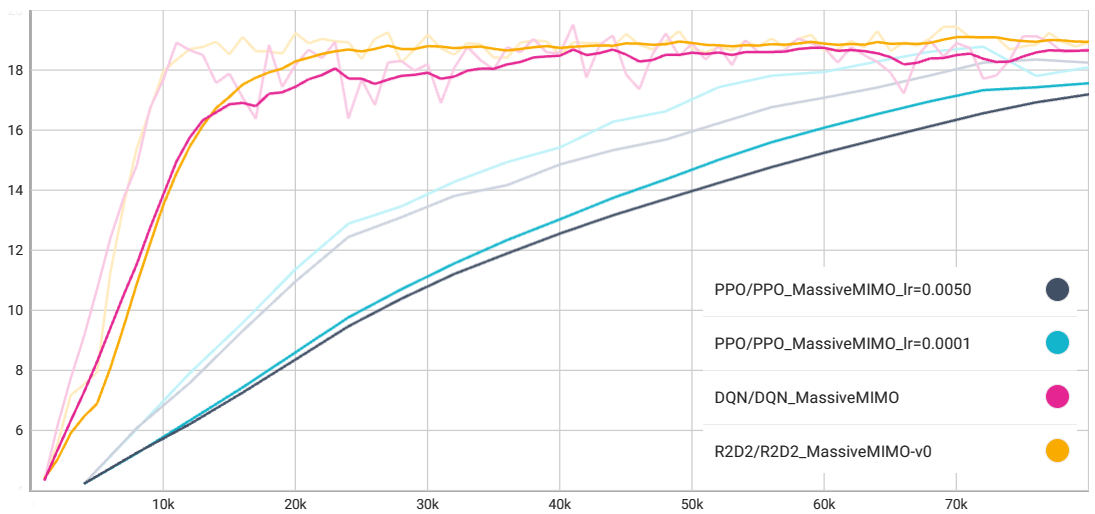
\includegraphics[width=0.48\textwidth, height=0.25\textwidth]{figures/Mean_Reward.png}
    \caption{Mean Episode Reward}
    \label{fig:meanr}
\end{figure}

The performance of the agents was evaluated based on three metrics: average episode reward, minimum episode reward, and stability of the learning process. Figure \ref{fig:meanr} displays the mean episode reward of the three agents over the training period. R2D2 demonstrated the most stable and fastest achievement of the desired reward. DQN nearly matched R2D2 in the speed of reaching the desired reward but exhibited inherent instability, as evidenced by the Temporal Difference (TD) error plot in Figure \ref{fig:dqntd}. On the other hand, PPO, which was trained with two different learning rates, achieved a comparable average reward but at a considerably later stage than the other agents.

\begin{figure}[t!]
    \centering
    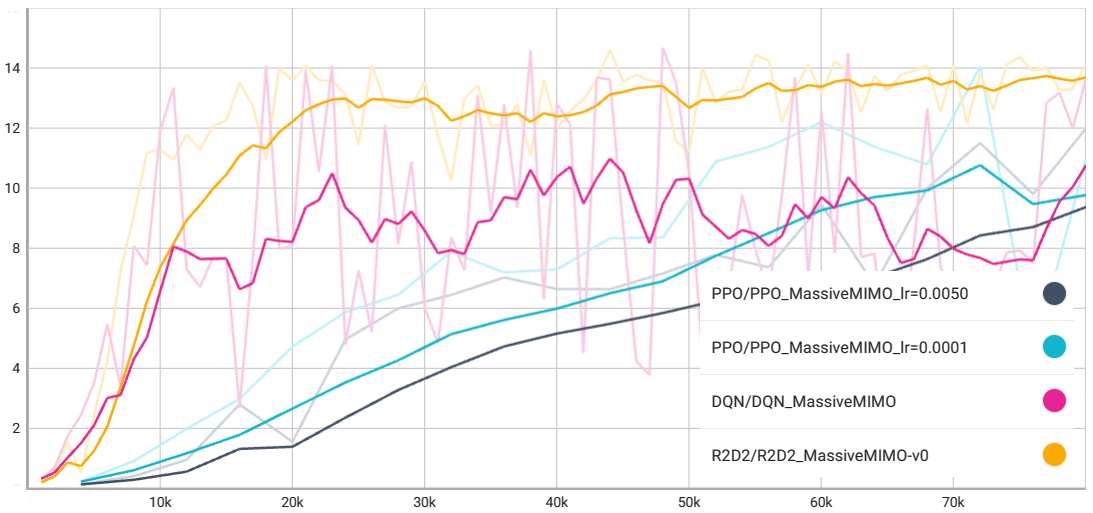
\includegraphics[width=0.48\textwidth, height=0.25\textwidth]{figures/Min_Reward.png}
    \caption{Minimum Episode Reward}
    \label{fig:minr}
\end{figure}

To further examine the agents' performance, we generated a plot of the minimum episode reward attained during training. As shown in Figure \ref{fig:minr}, R2D2 achieved the highest minimum episode reward, followed by DQN, while PPO had the lowest minimum episode reward. This superior performance of R2D2 can be attributed to its double DQN architecture, which mitigates overfitting issues that can arise when the agent predicts Q-values for unseen states. Additionally, the prioritized experience replay buffer used by R2D2 ensures that the agent learns from the most critical experiences, leading to faster and more accurate learning. As a result, R2D2 learns to estimate the value of each state and action more accurately.

\begin{figure}[b!]
    \centering
    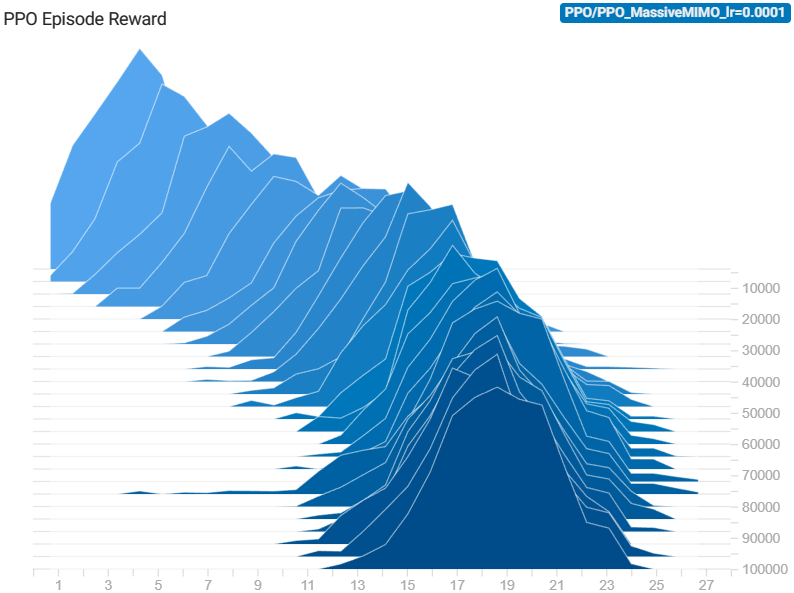
\includegraphics[width=0.48\textwidth, height=0.35\textwidth]{figures/PPO_Reward.png}
    \caption{PPO Reward Histogram}
    \label{fig:ppor}
\end{figure}

The reward distribution of the trained agents was analyzed using histograms, which are presented in Figure \ref{fig:ppor}, \ref{fig:dqnr}, and \ref{fig:r2d2r} for PPO, DQN, and R2D2, respectively. The reward distribution of R2D2 is the most concentrated around the desired reward, indicating a more stable learning process. On the other hand, DQN shows a wider range of reward distribution, which can be attributed to its inherent instability. PPO, while showing a stable reward distribution, is the slowest of the implemented techniques, as previously shown in the mean episode reward and minimum episode reward plots in Figure \ref{fig:meanr} and Figure \ref{fig:minr}, respectively. These results suggest that R2D2 is the most effective agent, with stable and fast convergence towards the optimal reward, followed by DQN, which may require additional training steps to reduce its inherent instability. Meanwhile, PPO, while showing potential for stable reward distribution, may require additional training time to reach optimal performance.

\begin{figure}[t!]
    \centering
    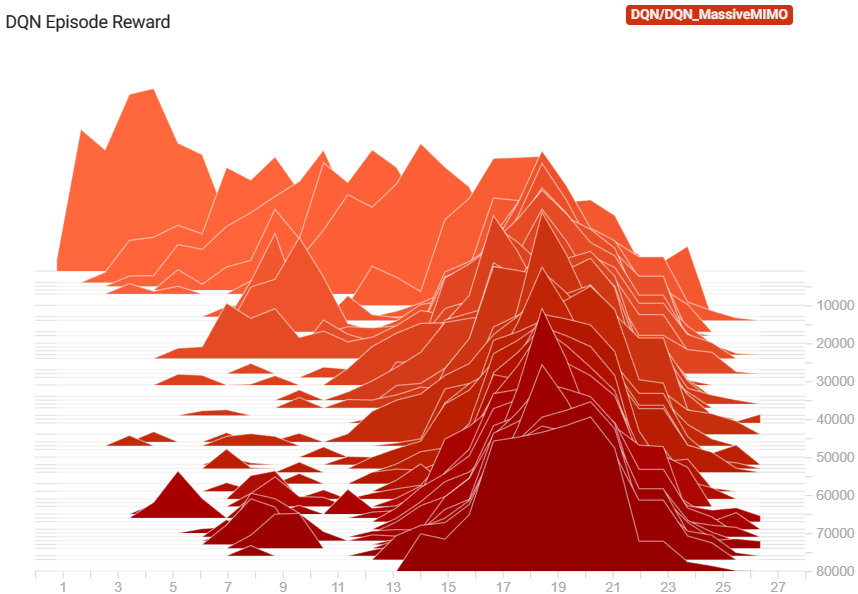
\includegraphics[width=0.48\textwidth, height=0.35\textwidth]{figures/DQN_Reward.png}
    \caption{DQN Reward Histogram}
    \label{fig:dqnr}
\end{figure}

\begin{figure}[t!]
    \centering
    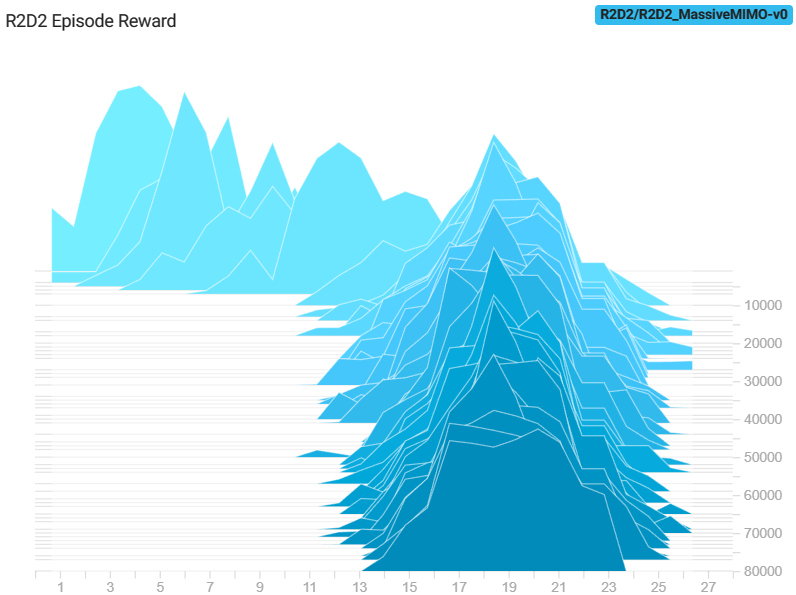
\includegraphics[width=0.48\textwidth, height=0.35\textwidth]{figures/R2D2_Reward.png}
    \caption{R2D2 Reward Histogram}
    \label{fig:r2d2r}
\end{figure}

To further investigate the instability of DQN, we plotted the TD error of the agent during training. Figure \ref{fig:dqntd} shows the TD error of DQN, which exhibits a high variance throughout the training process, indicating instability. In contrast, R2D2 exhibits a relatively stable TD error as shown in Figure \ref{fig:r2d2td}. This is because R2D2 uses a double DQN architecture, a prioritized experience replay buffer, and a dueling DQN architecture. These improvements help R2D2 to learn more quickly and more accurately than DQN. During training, DQN is known to suffer from bootstrapping bias because it updates the Q-value of the current state using the Q-value of the next state, which is only an estimate. This leads to overconfident Q-value predictions. On the other hand, R2D2 uses a double DQN architecture, which involves two Q-networks. The first network estimates the Q-value of the next state while the second network predicts the Q-value of the current state. This reduces bootstrapping bias as the second Q-network does not have access to the Q-value of the next state.

\begin{figure}[b!]
    \centering
    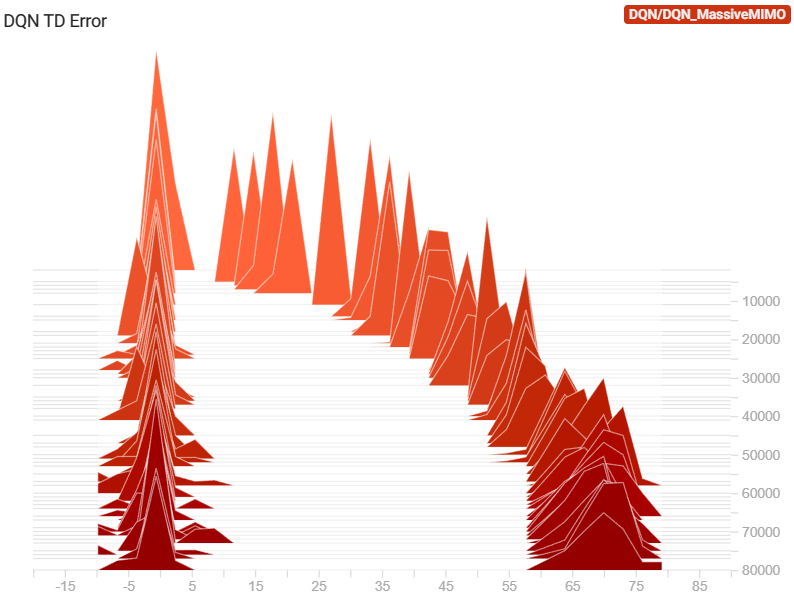
\includegraphics[width=0.48\textwidth, height=0.35\textwidth]{figures/DQN_TD.png}
    \caption{DQN TD Error}
    \label{fig:dqntd}
\end{figure}

\begin{figure}[b!]
    \centering
    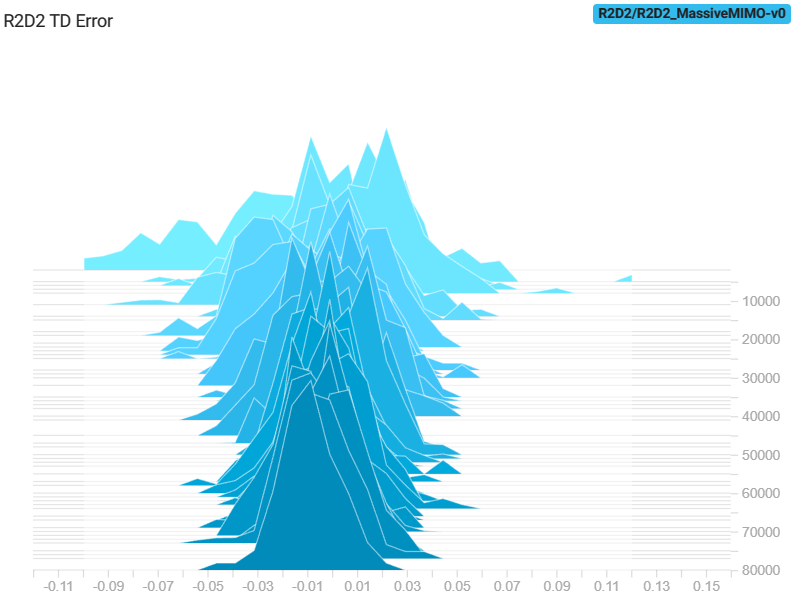
\includegraphics[width=0.48\textwidth, height=0.35\textwidth]{figures/R2D2_TD.png}
    \caption{R2D2 TD Error}
    \label{fig:r2d2td}
\end{figure}

Our study has shown that the R2D2 algorithm outperforms the other agents in terms of both stability and speed of achieving the desired reward for dynamic resource allocation in wireless networks. Although DQN performs comparably in achieving the desired reward, it suffers from inherent instability, as evident from the TD error plot. PPO, trained with two separate learning rates, achieves lower performance in terms of both the desired reward and the stability of the learning process when compared to the other agents.

\section{Conclusion}
In this report, we investigated the application of deep reinforcement learning (DRL) algorithms for dynamic resource allocation in wireless communication systems. We created a simulation environment that models a wireless network with dynamic resource allocation and utilized the RLlib library to compare the performance of two popular DRL algorithms, namely DQN and PPO. Our results show that the choice of algorithm and learning rate significantly affect the system's performance, and the use of DRL algorithms can provide more efficient resource allocation compared to traditional methods.

Specifically, our experiments show that R2D2, a variant of DQN, outperforms both DQN and PPO in terms of achieving the desired reward most stably and the fastest. Our results also highlight the importance of choosing an appropriate learning rate, as the use of two separate learning rates in PPO did not improve its performance compared to using a single learning rate.

\bibliographystyle{IEEEtran}
\bibliography{ref}
	
\end{document}